\documentclass[11pt,a4paper,fontset=fandol]{ctexart}

\usepackage{amsmath,amssymb,bm}
\usepackage{geometry}
\usepackage{enumitem}
\usepackage{fancyhdr}
\usepackage{lastpage}
\usepackage{xcolor}
\usepackage[most]{tcolorbox}
\usepackage{titlesec}
\usepackage{graphicx}
\usepackage{booktabs}
\usepackage{array}

\geometry{left=2.15cm,right=2.15cm,top=2.0cm,bottom=2.0cm}
\setlength{\parindent}{2em}
\setlength{\parskip}{0.22em}
\linespread{1.10}

\definecolor{mainblue}{RGB}{39,91,150}
\definecolor{lightblue}{RGB}{232,241,252}
\definecolor{darkgray}{RGB}{65,65,65}
\definecolor{lightgray}{RGB}{245,246,248}
\definecolor{warn}{RGB}{156,87,34}
\definecolor{softgreen}{RGB}{236,246,238}
\definecolor{deepgreen}{RGB}{63,123,74}

\titleformat{\section}{\large\bfseries\color{mainblue}}{}{0em}{}[\titlerule]
\titleformat{\subsection}{\normalsize\bfseries\color{darkgray}}{}{0em}{}
\titlespacing*{\section}{0pt}{0.85em}{0.42em}
\titlespacing*{\subsection}{0pt}{0.62em}{0.22em}

\setlist[enumerate]{leftmargin=2.2em,itemsep=0.22em,topsep=0.22em}
\setlist[itemize]{leftmargin=2.0em,itemsep=0.18em,topsep=0.18em}

\pagestyle{fancy}
\fancyhf{}
\lhead{\small 格物助航｜每日一练}
\rhead{\small 2026.6.14}
\cfoot{\small 第 \thepage\ 页 / 共 \pageref{LastPage} 页}
\renewcommand{\headrulewidth}{0.4pt}

\newtcolorbox{problemBox}{
 colback=lightblue,
 colframe=mainblue,
 arc=2mm,
 boxrule=0.7pt,
 left=1.0em,
 right=1.0em,
 top=0.75em,
 bottom=0.75em,
 before skip=0.55em,
 after skip=0.75em
}

\newtcolorbox{tipBox}{
 colback=lightgray,
 colframe=darkgray,
 arc=1.5mm,
 boxrule=0.5pt,
 left=0.9em,
 right=0.9em,
 top=0.55em,
 bottom=0.55em,
 before skip=0.45em,
 after skip=0.45em
}

\newtcolorbox{warnBox}{
 colback=white,
 colframe=warn,
 arc=1.5mm,
 boxrule=0.6pt,
 left=0.9em,
 right=0.9em,
 top=0.55em,
 bottom=0.55em,
 before skip=0.45em,
 after skip=0.45em
}

\newtcolorbox{ideaBox}{
 colback=softgreen,
 colframe=deepgreen,
 arc=1.5mm,
 boxrule=0.6pt,
 left=0.9em,
 right=0.9em,
 top=0.55em,
 bottom=0.55em,
 before skip=0.45em,
 after skip=0.45em
}

\newcommand{\dd}{\mathrm{d}}
\newcommand{\eps}{\varepsilon_0}
\graphicspath{{fig_6.14/}}

\begin{document}

\begin{center}
 {\Large\bfseries\color{mainblue} 格物助航｜每日一练}\par
 \vspace{0.25em}
 {\large 电磁学第一章：静电场}\par
 \vspace{0.35em}
 {\small 2026年6月14日}\par
 \vspace{0.35em}
 {\small 编写：拯救世界的大小王}
\end{center}

\vspace{-0.3em}

\begin{problemBox}
\noindent\textbf{题目：八分之一均匀带电球体在球心处的电场}\quad
如图所示，把半径为 $R$ 的球体切为八等份，取其中一份，做均匀带电，电荷体密度为 $\rho$。试求此八分之一带电球体在球心 $O$ 处的电场强度大小 $E_0$。

\begin{center}
 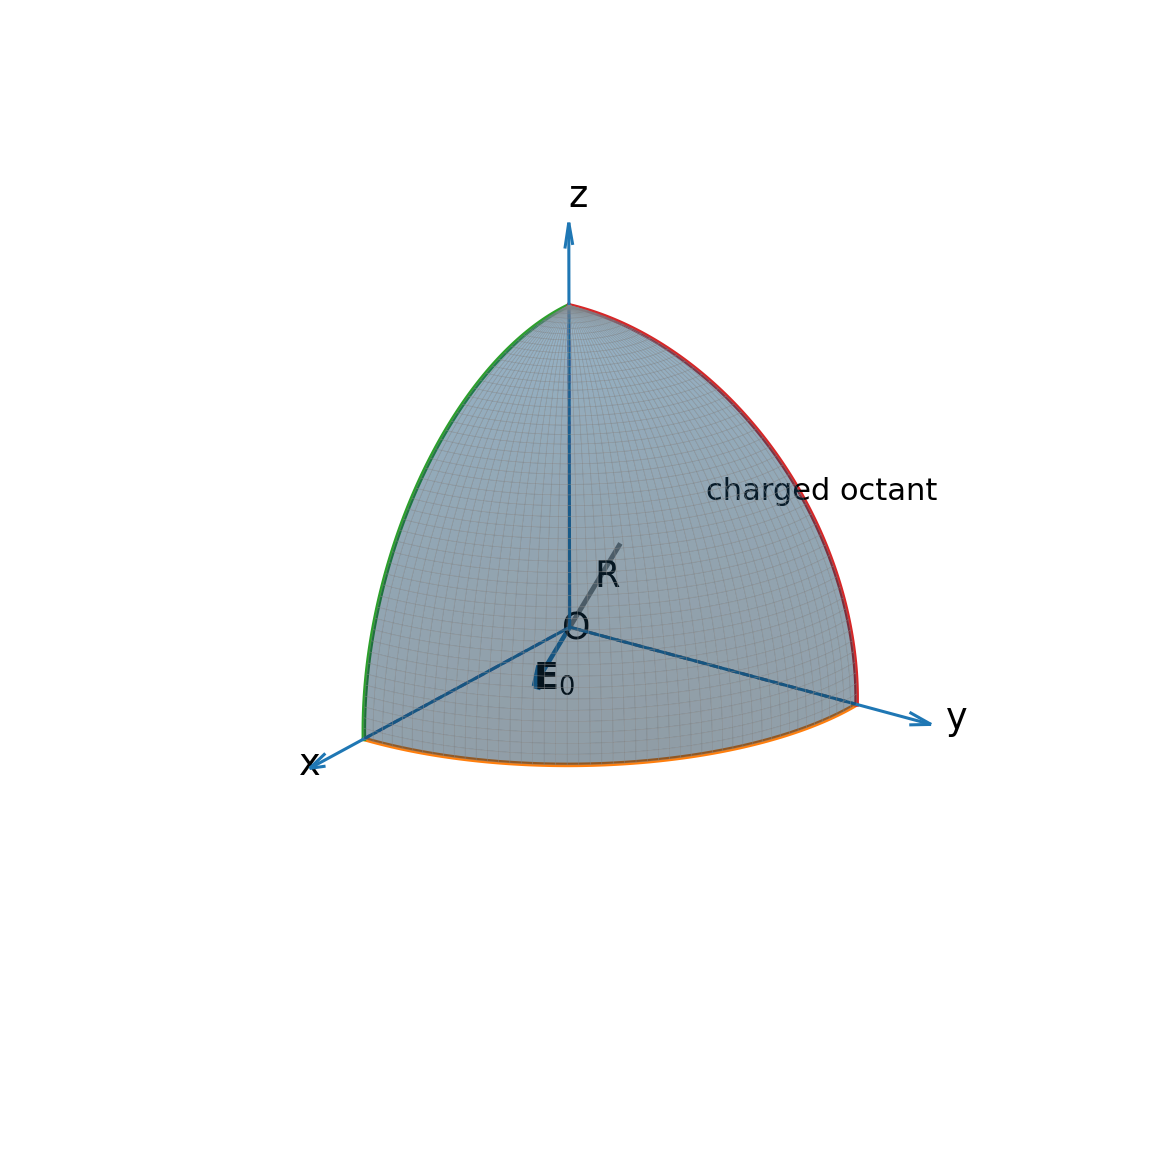
\includegraphics[width=0.68\linewidth]{fig_6.14/2026.6.14.png}

 {\small 图1\quad 八分之一均匀带电球体及球心处电场方向示意}
\end{center}
\end{problemBox}

\section*{题目分析}
\begin{ideaBox}
这道题看起来像球形带电体问题，但它不是完整均匀带电球。只有八分之一球体带电，完整球对称性被破坏，因此不能直接套用均匀带电球内部场强公式，也不能直接用一个球形高斯面求出 $E_0$。

本题的关键思想是把三维体电荷分布拆成两步处理。第一步，先求一个八分之一均匀带电球面在球心处产生的电场。第二步，把八分之一带电球体看成许多很薄的八分之一球面叠加，再沿半径方向积分。
\end{ideaBox}

\section*{详细解法}

\subsection*{一、为什么不能直接用高斯定理求场强}
高斯定理为
\begin{equation}
 \oint_S \bm E\cdot \dd \bm S=\frac{q_{\mathrm{in}}}{\eps}.
 \label{eq:gauss-law}
\end{equation}

式 \eqref{eq:gauss-law} 对任何静电场都成立，但它只能给出闭合曲面上的电通量。若想进一步由通量直接得到场强大小，必须依靠足够强的对称性，使得某个高斯面上 $E$ 的大小和方向都可以被简化。

本题只有八分之一球体带电，不具有完整球对称性。球心处电场不为零，简单球面上场强大小也不处处相等。因此，高斯定理不能直接求出 $E_0$。本题应使用叠加原理与对称性分析。

\subsection*{二、先求八分之一均匀带电球面在球心处的电场}
设有一个半径为 $r$ 的八分之一球面，面电荷密度为常量 $\sigma$。取球面上的一个面元 $\dd S$，它在球心 $O$ 处产生的电场大小为
\begin{equation}
 \dd E=\frac{1}{4\pi\eps}\frac{\sigma\dd S}{r^2}.
 \label{eq:dE-surface}
\end{equation}

若带电部分位于第一卦限，正电荷在球心处产生的电场指向远离带电区域的方向，即沿空间对角线反方向。由于八分之一球面对 $x,y,z$ 三个方向完全对称，球心处电场的三个分量大小相等：
\begin{equation}
 |E_x|=|E_y|=|E_z|.
 \label{eq:component-equal}
\end{equation}

下面求 $x$ 方向分量的大小。设面元法线与 $x$ 轴的夹角为 $\alpha$，则
\begin{equation}
 \dd E_x^{\ast}=\dd E\cos\alpha
 =\frac{1}{4\pi\eps}\frac{\sigma\dd S}{r^2}\cos\alpha.
 \label{eq:dEx-surface}
\end{equation}

其中 $\dd S\cos\alpha$ 是面元在垂直于 $x$ 轴的平面上的投影面积。整个八分之一球面投影到 $yz$ 平面上，得到一个半径为 $r$ 的四分之一圆面，因此
\begin{equation}
 \int \dd S\cos\alpha=\frac{\pi r^2}{4}.
 \label{eq:projection-area}
\end{equation}

由式 \eqref{eq:dEx-surface} 与式 \eqref{eq:projection-area} 得
\begin{equation}
 |E_x|=\frac{1}{4\pi\eps}\frac{\sigma}{r^2}\cdot\frac{\pi r^2}{4}
 =\frac{\sigma}{16\eps}.
 \label{eq:Ex-surface}
\end{equation}

同理，
\begin{equation}
 |E_y|=|E_z|=\frac{\sigma}{16\eps}.
 \label{eq:EyEz-surface}
\end{equation}

所以，八分之一均匀带电球面在球心处产生的电场大小为
\begin{equation}
 E_{\mathrm{surf}}
 =\sqrt{E_x^2+E_y^2+E_z^2}
 =\frac{\sqrt3\sigma}{16\eps}.
 \label{eq:surface-field-size}
\end{equation}

若该八分之一球面位于第一卦限，且 $\sigma>0$，其电场矢量为
\begin{equation}
 \bm E_{\mathrm{surf}}
 =-\frac{\sigma}{16\eps}\left(\bm i+\bm j+\bm k\right).
 \label{eq:surface-field-vector}
\end{equation}

\subsection*{三、由八分之一球面叠加成八分之一球体}
现在回到原题。八分之一带电球体的体电荷密度为 $\rho$，可以把它看成许多半径为 $r$、厚度为 $\dd r$ 的薄八分之一球壳叠加而成。

对其中一个薄球壳而言，它的体电荷可以等效为一层很薄的球面电荷，其等效面电荷密度为
\begin{equation}
 \dd \sigma=\rho\dd r.
 \label{eq:equivalent-sigma}
\end{equation}

把式 \eqref{eq:equivalent-sigma} 代入式 \eqref{eq:surface-field-size}，这一薄八分之一球壳在球心处产生的电场大小为
\begin{equation}
 \dd E_0=\frac{\sqrt3}{16\eps}\dd\sigma
 =\frac{\sqrt3\rho}{16\eps}\dd r.
 \label{eq:dE-shell}
\end{equation}

所有薄八分之一球壳在球心处产生的电场方向相同，均沿带电区域所在空间对角线的反方向。因此可以直接对大小积分：
\begin{equation}
 E_0=\int_0^R\dd E_0
 =\int_0^R\frac{\sqrt3\rho}{16\eps}\dd r
 =\frac{\sqrt3\rho R}{16\eps}.
 \label{eq:final-size-rho}
\end{equation}

因此，本题所求电场强度大小为
\begin{equation}
 \boxed{E_0=\frac{\sqrt3\rho R}{16\eps}}.
 \label{eq:boxed-answer}
\end{equation}

若进一步写出方向，并假设带电部分位于第一卦限且 $\rho>0$，则
\begin{equation}
 \bm E_0=-\frac{\rho R}{16\eps}\left(\bm i+\bm j+\bm k\right).
 \label{eq:final-vector-rho}
\end{equation}

式 \eqref{eq:final-vector-rho} 的大小正是式 \eqref{eq:boxed-answer}。

\section*{答案汇总}
\begin{ideaBox}
\begin{enumerate}
 \item 八分之一均匀带电球面在球心处的电场大小为
 \[
 E_{\mathrm{surf}}=\frac{\sqrt3\sigma}{16\eps}.
 \]
 \item 八分之一均匀带电球体在球心处的电场强度大小为
 \[
 E_0=\frac{\sqrt3\rho R}{16\eps}.
 \]
 \item 若带电部分位于第一卦限且 $\rho>0$，则电场方向沿 $-(\bm i+\bm j+\bm k)$，也就是指向第三卦限方向。
\end{enumerate}
\end{ideaBox}

\section*{技巧与知识点}
\begin{tipBox}
\begin{enumerate}
 \item \textbf{高斯定理不是不能用，而是不能直接用来求场强。} 它可以给出通量，但本题缺少完整球对称性，不能把通量简单写成 $E$ 乘面积。
 \item \textbf{先面后体是本题的核心降维策略。} 先求八分之一带电球面，再把球体拆成许多薄球面叠加，三维体积分就变成一维半径积分。
 \item \textbf{投影面积法可以避开复杂积分。} 求 $x$ 分量时，$\dd S\cos\alpha$ 正是面元投影面积，整个八分之一球面投影成四分之一圆面。
 \item \textbf{矢量方向由对称性决定。} 三个分量大小相等，方向沿空间对角线。若正电荷位于第一卦限，球心处电场指向第三卦限。
 \item \textbf{薄壳等效面密度容易写错。} 厚度为 $\dd r$ 的薄球壳满足 $\dd\sigma=\rho\dd r$，这里不需要额外乘 $r$ 或 $r^2$。
\end{enumerate}
\end{tipBox}

\section*{常见误区}
\begin{warnBox}
\begin{enumerate}
 \item \textbf{误区一：看到球体就套完整均匀带电球公式。} 完整球体在球心处电场为零，是因为各方向完全抵消。本题只有八分之一球体带电，抵消关系不存在。
 \item \textbf{误区二：把高斯定理当成万能求场强公式。} 高斯定理总是成立，但只有在场强分布高度对称时才能直接解出 $E$。
 \item \textbf{误区三：只算大小，忘记方向。} 本题虽然问大小，但理解方向才能保证分量关系和符号没有错。
 \item \textbf{误区四：把球壳面积因子重复计算。} 在先面后体法中，八分之一球面结论已经包含了球面面积信息，向体分布过渡时只需要写 $\dd\sigma=\rho\dd r$。
\end{enumerate}
\end{warnBox}

\section*{备考建议}
\begin{tipBox}
\begin{enumerate}
 \item \textbf{先判断对称性，再选方法。} 静电场题目不要一上来就列高斯定理。先问自己电荷分布是否具有球对称、柱对称或面对称。如果没有足够对称性，就优先考虑叠加法。
 \item \textbf{把高斯定理和叠加法分清楚。} 高斯定理适合完整球、无限长圆柱、无限大平面这类高对称模型；叠加法适合圆环、圆盘、半球面、八分之一球体这类不完整分布。
 \item \textbf{重点练投影面积法。} 遇到球面上求某一方向分量时，不一定要写复杂角积分。把 $\dd S\cos\alpha$ 看成投影面积，往往能迅速化简。
 \item \textbf{复习时建立模型链条。} 建议按点电荷、圆环、圆盘、球面、半球面、八分之一球面、八分之一球体的顺序复习。这样能看清叠加思想如何一步步升级。
 \item \textbf{答案检查要看量纲和极限。} 本题结果 $E_0$ 与 $\rho R/\eps$ 成正比，量纲正确；半径越大，沿同一方向叠加的薄球壳越多，场强越大，也符合直觉。
 \item \textbf{考试中保留关键解释。} 这类题不能只写积分结果。建议至少写出不能直接用高斯定理的原因、八分之一球面中三个分量相等、以及由薄球壳叠加到球体这三句话。
\end{enumerate}
\end{tipBox}

\end{document}
